%!TEX root=../main.tex

\section*{Аннотация}

DSLab - программный фреймворк для имитационного моделирования и тестирования распределенных систем.

В проекте используется дискретно-событийный подход описания моделей и приложений, где события обрабатываются в пользовательских функциях (callback-ах). В рамках проекта предстоит добавить возможность управлять событиями асинхронно.


\section{Описание проекта и постановка задачи}

\subsection{Устройство DSLab}

В силу широты охвата областей применения фреймворка он организован в виде набора слабо связанных программных модулей, использование которых будет осуществляться через их API. Это даст возможность пользователям фреймворка (исследователям, разработчикам, преподавателям) гибким образом собирать из модулей решения под свои цели, например симуляторы для конкретных типов систем или постановок задач.

Входящие в состав фреймворка модули можно условно разделить на три типа:
\begin{enumerate}
    \item 
    Базовые, функциональность которых используется остальными модулями (например, 
    
    реализация дискретно-событийного моделирования)
    \item
    Универсальные, функциональность которых может быть использована в различных предметных областях (например, модели сети);
    \item
    Специализированные, которые заточены под определенную предметную область (например, библиотеки для моделирования облачных инфраструктур, исследования алгоритмов планирования заданий на кластерах или тестирования решений учебных заданий).
\end{enumerate}

Архитектуру DSLab можно схематично представить в виде трех слоев (Рис. \ref{dslab_arc}), включающих модули соответствующего типа. На рисунке также указаны текущие модули и зависимости между ними. Зависимости от dslab-core (от него зависят все имеющиеся универсальные и специализированные модули) не указаны, чтобы не загромождать рисунок. Таким образом, модули могут зависеть от модулей с нижних слоев, но не наоборот.

\begin{figure}[H]
    \centering
    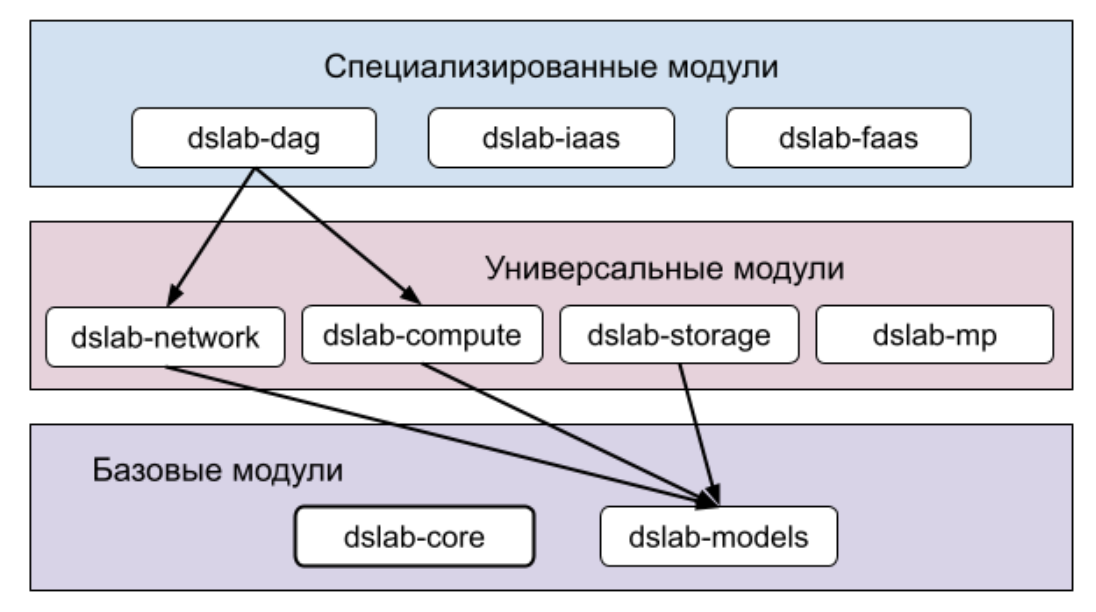
\includegraphics[width=0.7\linewidth]{images/dslab_arc.png}
    \caption{Архитектура DSLab}
    \label{dslab_arc}
\end{figure}

Описание архитектуры основано на документации проекта \cite{dslab-architecture}. Более подробно про проект можно прочитать в его описании \cite{dslab-description}, его требования \cite{dslab-requirements} и сравнение с аналогами \cite{dslab-analog-cmp}. Реализации модулей представлены в репозитории \cite{dslab-repo}.

Таким образом пользователь при разработке собственной симуляции может либо использовать уже готовые разработанные компоненты, либо реализовывать свои и произвольно их связывать. 


Основным процессом создания симуляции является создание событий и написание процессов реагирования на них. Каждое событие представляет из себя следующую структуру: 
\begin{enumerate}
    \item идентификатор события 
    \item идентификатор компонента, создавшего событие 
    \item идентификатор компонента, которому это событие предназначено доставить 
    \item внутреннее время, когда событие должно наступить
    \item произвольные данные события (<<полезная нагрузка>>)
\end{enumerate}

Таким образом в процессе симуляции разные компоненты генерируют события друг для друга и с помощью низкоуровневого модуля dslab-core обмениваются ими. Чтобы как-то реагировать на событие, каждый компонент реализует единственный обобщенный метод в который dslab-core передает нужное событие. При обработке события компоненты генерируют новые и таким образом цикл симуляции замыкается. 

Получается, что сейчас реагировать на пришедшие события можно только в одном месте -- в той самой функции-callback которую позовет dslab-core. В случае, когда событий немного -- это лаконично выглядит и этим удобно пользоваться. Но в более сложных алгоритмах с большим количеством различных событий, и, что важнее, цепочками событий, на которые нужно последовательно реагировать, подобная модель становится не самой удобной. С такой единой точной входа многие последовательные логичные действия оказываются фрагментированы (разбросаны по разным участкам кода). 

Хотелось бы иметь альтернативную возможность писать на языке программирования более понятный с первого взгляда алгоритм.

Как раз такой возможностью является написание асинхронного кода. Тогда различные сложные куски логики можно было бы выносить в отдельные функции, держать их вместе, просто исполнение бы прерывалось в ожидании какого-то события, чтобы продолжить.

\subsection{Цель}

Добавить возможность пользователю использовать асинхронность при программировании симуляции в DSLab.

\subsection{Задачи}
\begin{itemize}
    \item Реализовать асинхронное расширение для существующего ядра dslab-core или реализовать альтернативное асинхронное ядро 
    \item Добавить примеры использования нового функционала высокоуровневыми компонентами
    \item Написать подробную документацию нового API и покрыть реализацию тестами.
\end{itemize}

\subsection{Требования}

\begin{itemize}
    \item Код нового ядра должен быть написан на языке Rust и опубликован как модуль проекта DSLab.
    \item Реализация должна корректно обрабатывать все возможные возникающие комбинации событий в асинхронном контексте. Все возможные случаи должны быть описаны в документации и покрыты тестами.
    \item Новое ядро должно быть реализовано эффективно: не должны возникать дополнительные накладные расходы по сравнению со стандартным ядром.
    \item Реализация должна содержать логирование происходящего в асинхронном контексте, а так же обработку ошибок, которая бы помогала пользователю искать ошибки в коде. 
    \item Работа нового ядра должна быть продемонстрирована в использовании на разработанных примерах симуляций, в которых используется стандартная callback-based модель. Должны быть описаны преимущества и недостатки нового подхода.
\end{itemize}

\section{Актуальность и значимость}

\subsection{Значимость проекта DSLab}

Практически все современные информационные и вычислительные системы являются распределенными. Связано это с растущими объемами вычислений и обрабатываемых данных, требованиями к производительности, надежности и масштабируемости. Алгоритмическое обеспечение распределенных систем (например, алгоритмы управления ресурсами, планирования задач, балансировки нагрузки, членства в группе, консенсуса) является предметом активных исследований. В силу масштабов современных систем, сложности их реализации и недетерминированного характера, исследование алгоритмов и тестирование их реализаций в реальных системах существенно затруднено. Поэтому часто подобные исследования проводятся на аналитических и имитационных моделях, описывающих существенные для решаемой задачи аспекты поведения системы и проводимых вычислений. Использование моделей позволяет значительно удешевить эксперименты, сократить время их проведения и обеспечить воспроизводимость их результатов \cite{dslab-description}. 

\subsection{Преимущества асинхронного подхода}

Как уже было описано в мотивации постановки цели этой работы, главное преимущество асинхронной модели~--~удобство при написании сложных многоступенчатых алгоритмов.

Это повысит читаемость кода. Процесс принятия решения о сохранении файла в распределенном хранилище в такой парадигме мог бы выглядеть таким образом (псевдокод):

\begin{figure}[H]
\begin{lstlisting}[language=Python]
    async fn add_file_to_storage(some_file) {
        send_file_to_all_replicas(some_file);
        result = wait_for_confirmation_from_all().await;
        if result.has_quorum {
            send_commit_to_all_replicas();
            wait_for_commit_confirmation_from_quorum().await;
            send_ok_message_to_user();
        } else {
            send_reject_message_to_user();
        }
    }
\end{lstlisting}
\caption{Псевдокод асинхронного взаимодействия нод в симуляции}
\label{pseudocode}
\end{figure}

Посмотрев на функцию можно понять, что она делает, потому что логика последовательна и удобно разбита на подфункции. У нас есть возможность написать такой алгоритм на верхнем уровне, а не обрабатывать сообщения всех типов от всех реплик в единой точке входа.

\subsection{Возможные недостатки асинхронного подхода}

Программировать в парадигме асинхронного взаимодействия требует соответствующей подготовки пользователя. Не смотря на то, что в любой момент времени исполняется только одна функция, и проблем многопоточного программирования вида \texttt{data-race} не возникает, нужно постоянно держать в голове, что <<параллельно>> могут быть запущены другие процессы, которые могли поменять общую память в то время, когда функция была неактивна. 

\section{Существующие работы и решения}

Подобный подход уже был реализован в других симуляторах, например в SimGrid \cite{simgrid-example}, но этот код сложно назвать легко читаемым, потому что SimGrid является низкоуровневым фреймворком.

Более близким к желаемой реализации является использование корутин языка Kotlin в проекте OpenDC~\cite{opendc-repo}. К сожалению, проект не содержит достаточно разнообразных примеров использования симуляции в асинхронном контексте, но простой пример запуска симуляции в асинхронном контексте~\cite{opendc-example} очень похож на ожидаемый опыт использования асинхронности в DSLab.


Опыт других проектов не очень хорошо подходит как опора для разработки нового решения из-за специфики языка Rust и внутренней архитектуры симулятора.

\section{Предлагаемые подходы и методы} 

\subsection{Изучение технологий}
В качестве знакомства с языком программирования Rust и его концепциями я прошел часть курса ШАД по расту \cite{shad-rust}. В нем особенно интересовала глава про асинхронное программирование. У Rust есть официальная документация по асинхронности.\cite{async-book}. Она еще не завершена, но основные идеи по написанию собственного рантайма там изложены.


\subsection{Написание прототипа}
Чтобы дать возможность пользователю писать асинхронный код, нужно создать саму возможность обрабатывать события асинхронно. Для этого нужно написать свой executor задач в DSLab, который будет исходя из внутренней логики (наступление времени, когда событие нужно доставить получателю) понимать, когда и какую асинхронную задачу нужно разбудить, и дать ей продолжить исполнение. 

Для этого нужно реализовать альтернативу dslab-core (или дополнить уже сущетсвующую реализацию), и затем уже пользоваться новым интерфейсом на более верхних уровнях. К счастью, язык Rust дает возможность пользователям самим управлять процессом рантайма: с помощью библиотеки futures \cite{rust-futures} такое поведение может быть реализовано (что на простом примере и описано в официальной документации \cite{async-book}).

Изучив предлагаемые там примеры и посмотрев материалы был реализован прототип \cite{my-demo}. Он поддерживает простой обмен сообщениями и ожидания прихода сообщений от других компьютеров в симуляции. Синтаксис, которым там можно оперировать, соответствует представленному превдокоду (Рис. \ref{pseudocode}). В качестве тестирования прототипа был написан пример реплицированного хранения данных на 3 нодах и процесс обмена разными типами сообщений между ними, чтобы поддерживать консистентное состояние \cite{my-demo-replicas}. 

В примере можно видеть, что управление симуляцией (постановка условий и задач для хранилища) так же осуществляется с помощью асинхронных функций. В этом тоже есть удобство: процесс симуляции пишется как сценарий, который легко читать. 

\subsection{Перенос прототипа в проект DSLab}

Основываясь на полученных результатах в процессе разработки прототипа, нужно встроить эту логику в DSLab. Для этого нужно перевести прототип на использование сущностей из DSLab-а, а также перенести пример использования нового асинхронного ядра и добавить другие примеры, иллюстрирующие данных подход, его преимущества и недостатки в сравнении с callback-based методом. 

По возможности хочется добиться совместимости уже написанных компонент с новым ядром, тем самым давая пользователю выбор между асинхронной моделью программирования и программирования на callback-ах. Этот вопрос предстоит исследовать. 

\section{Ожидаемые результаты}

\begin{enumerate}
    \item 
    Основным результатом проекта будет конкретный программный артефакт, в виде нового или расширенного ядра и API симуляции в DSLab, позволяющий пользователю писать собственные модули и симуляции в асинхронной модели. 
    \item В репозиторий DSLab \cite{dslab-repo} добавлены примеры кода, документация по использованию асинхронного ядра.
    \item Реализация покрыта тестами.
\end{enumerate}
    
\section{План работ}

Стратегия разработки совпадает со стандартным процессом создания программного продукта 

\begin{table}[!h]
	\centering
\begin{tabular}{|l|p{27em}|c|}
	\hline
№	& Описание этапа &  Примерный срок выполнения \\
	\hline
	1 & Работа с источниками, изучение Rust &  01.11.2022 --- 31.01.2023\\ 
	\hline
2 & Реализация прототипа асинхронного ядра и примеров его использования & 01.12.2022 --- 31.01.2023 \\
	\hline
3	& Перенос прототипа асинхронного ядра в DSLab, написание примеров &  01.02.2023 --- 30.03.2023 \\
\hline
4	& Исследование возможностей совмещения двух парадигм разработки внутри одного модуля &  01.03.2023 --- 30.03.2023 \\
	\hline
5	& Тестирование всех функций и написание документации &  01.04.2022 --- 30.04.2023  \\
	\hline
6	& Написание отчетных документов и подготовка к защите & 01.05.2023 --- 15.05.2023 \\
	\hline
\end{tabular}
	\caption{Ожидаемые сроки выполнения}
	\label{table1}
\end{table}

